% Options for packages loaded elsewhere
\PassOptionsToPackage{unicode}{hyperref}
\PassOptionsToPackage{hyphens}{url}
\PassOptionsToPackage{dvipsnames,svgnames,x11names}{xcolor}
%
\documentclass[
  letterpaper,
  DIV=11,
  numbers=noendperiod]{scrartcl}

\usepackage{amsmath,amssymb}
\usepackage{iftex}
\ifPDFTeX
  \usepackage[T1]{fontenc}
  \usepackage[utf8]{inputenc}
  \usepackage{textcomp} % provide euro and other symbols
\else % if luatex or xetex
  \usepackage{unicode-math}
  \defaultfontfeatures{Scale=MatchLowercase}
  \defaultfontfeatures[\rmfamily]{Ligatures=TeX,Scale=1}
\fi
\usepackage{lmodern}
\ifPDFTeX\else  
    % xetex/luatex font selection
\fi
% Use upquote if available, for straight quotes in verbatim environments
\IfFileExists{upquote.sty}{\usepackage{upquote}}{}
\IfFileExists{microtype.sty}{% use microtype if available
  \usepackage[]{microtype}
  \UseMicrotypeSet[protrusion]{basicmath} % disable protrusion for tt fonts
}{}
\makeatletter
\@ifundefined{KOMAClassName}{% if non-KOMA class
  \IfFileExists{parskip.sty}{%
    \usepackage{parskip}
  }{% else
    \setlength{\parindent}{0pt}
    \setlength{\parskip}{6pt plus 2pt minus 1pt}}
}{% if KOMA class
  \KOMAoptions{parskip=half}}
\makeatother
\usepackage{xcolor}
\setlength{\emergencystretch}{3em} % prevent overfull lines
\setcounter{secnumdepth}{-\maxdimen} % remove section numbering
% Make \paragraph and \subparagraph free-standing
\makeatletter
\ifx\paragraph\undefined\else
  \let\oldparagraph\paragraph
  \renewcommand{\paragraph}{
    \@ifstar
      \xxxParagraphStar
      \xxxParagraphNoStar
  }
  \newcommand{\xxxParagraphStar}[1]{\oldparagraph*{#1}\mbox{}}
  \newcommand{\xxxParagraphNoStar}[1]{\oldparagraph{#1}\mbox{}}
\fi
\ifx\subparagraph\undefined\else
  \let\oldsubparagraph\subparagraph
  \renewcommand{\subparagraph}{
    \@ifstar
      \xxxSubParagraphStar
      \xxxSubParagraphNoStar
  }
  \newcommand{\xxxSubParagraphStar}[1]{\oldsubparagraph*{#1}\mbox{}}
  \newcommand{\xxxSubParagraphNoStar}[1]{\oldsubparagraph{#1}\mbox{}}
\fi
\makeatother


\providecommand{\tightlist}{%
  \setlength{\itemsep}{0pt}\setlength{\parskip}{0pt}}\usepackage{longtable,booktabs,array}
\usepackage{calc} % for calculating minipage widths
% Correct order of tables after \paragraph or \subparagraph
\usepackage{etoolbox}
\makeatletter
\patchcmd\longtable{\par}{\if@noskipsec\mbox{}\fi\par}{}{}
\makeatother
% Allow footnotes in longtable head/foot
\IfFileExists{footnotehyper.sty}{\usepackage{footnotehyper}}{\usepackage{footnote}}
\makesavenoteenv{longtable}
\usepackage{graphicx}
\makeatletter
\def\maxwidth{\ifdim\Gin@nat@width>\linewidth\linewidth\else\Gin@nat@width\fi}
\def\maxheight{\ifdim\Gin@nat@height>\textheight\textheight\else\Gin@nat@height\fi}
\makeatother
% Scale images if necessary, so that they will not overflow the page
% margins by default, and it is still possible to overwrite the defaults
% using explicit options in \includegraphics[width, height, ...]{}
\setkeys{Gin}{width=\maxwidth,height=\maxheight,keepaspectratio}
% Set default figure placement to htbp
\makeatletter
\def\fps@figure{htbp}
\makeatother

\KOMAoption{captions}{tableheading}
\makeatletter
\@ifpackageloaded{caption}{}{\usepackage{caption}}
\AtBeginDocument{%
\ifdefined\contentsname
  \renewcommand*\contentsname{Table of contents}
\else
  \newcommand\contentsname{Table of contents}
\fi
\ifdefined\listfigurename
  \renewcommand*\listfigurename{List of Figures}
\else
  \newcommand\listfigurename{List of Figures}
\fi
\ifdefined\listtablename
  \renewcommand*\listtablename{List of Tables}
\else
  \newcommand\listtablename{List of Tables}
\fi
\ifdefined\figurename
  \renewcommand*\figurename{Figure}
\else
  \newcommand\figurename{Figure}
\fi
\ifdefined\tablename
  \renewcommand*\tablename{Table}
\else
  \newcommand\tablename{Table}
\fi
}
\@ifpackageloaded{float}{}{\usepackage{float}}
\floatstyle{ruled}
\@ifundefined{c@chapter}{\newfloat{codelisting}{h}{lop}}{\newfloat{codelisting}{h}{lop}[chapter]}
\floatname{codelisting}{Listing}
\newcommand*\listoflistings{\listof{codelisting}{List of Listings}}
\makeatother
\makeatletter
\makeatother
\makeatletter
\@ifpackageloaded{caption}{}{\usepackage{caption}}
\@ifpackageloaded{subcaption}{}{\usepackage{subcaption}}
\makeatother

\ifLuaTeX
  \usepackage{selnolig}  % disable illegal ligatures
\fi
\usepackage{bookmark}

\IfFileExists{xurl.sty}{\usepackage{xurl}}{} % add URL line breaks if available
\urlstyle{same} % disable monospaced font for URLs
\hypersetup{
  pdftitle={assignement\_gretl.qmd},
  pdfauthor={KLBRHBAY},
  colorlinks=true,
  linkcolor={blue},
  filecolor={Maroon},
  citecolor={Blue},
  urlcolor={Blue},
  pdfcreator={LaTeX via pandoc}}


\title{assignement\_gretl.qmd}
\author{KLBRHBAY}
\date{}

\begin{document}
\maketitle

\renewcommand*\contentsname{Table of contents}
{
\hypersetup{linkcolor=}
\setcounter{tocdepth}{3}
\tableofcontents
}
\listoffigures
\listoftables


\includegraphics{images/Skjermbilde 2026-03-10 115720.png} \newpage{}

\section{Step B: Analysis}\label{step-b-analysis}

\section{\texorpdfstring{\textbf{1:} Data Description \&
Summary}{1: Data Description \& Summary}}\label{data-description-summary}

Research question (RQ): We aim to investigate the determinants of
mortality rates across U.S. states.\\
Our research question is: ``To what extent do socioeconomic factors \&
health-related behaviors influence mortality rates across states?''.~

We use a cross-sectional dataset containing state-level data on
mortality rates, income, poverty, education, alcohol consumption,
cigarette consumption, healthcare expenditure, physicians per capita,
urbanization, \& age distribution. The dependent variable is total
mortality rate per 100,000 population. The independent variables include
socioeconomic indicators and health behavior variables suitable for
simple and multiple regression analysis. We have found this data on
Gretl itself, under Ramanathan, the name for the file is: data4-12
Mortality rates across states.

Summary statistics:

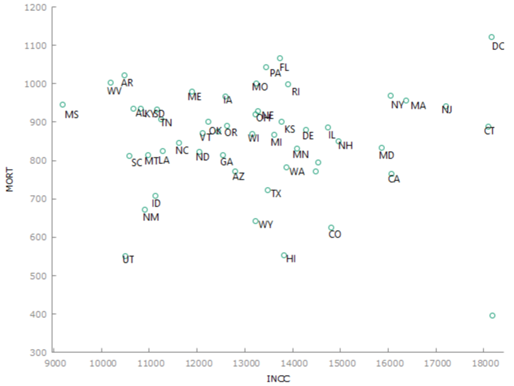
\includegraphics{images/Bilde2.png}

The dataset consists of 51 cross-sectional observations (all 50 states
plus District of Columbia), with no missing values. The dependent
variable MORT (mortality rates per 100~000 population), has a mean of
855,01 and a standard deviation of 137,97, ranging from 396,20 to
1120,5. The coefficient of variation is 0,16136 in the dependent
variable. This is relevant for the research question because mortality
rates vary meaningfully across states, making simple and multiple
regression model analysis appropriate. \newpage{}

\section{\texorpdfstring{\textbf{2. Simple Regression
Model}}{2. Simple Regression Model}}\label{simple-regression-model}

\textbf{a)}

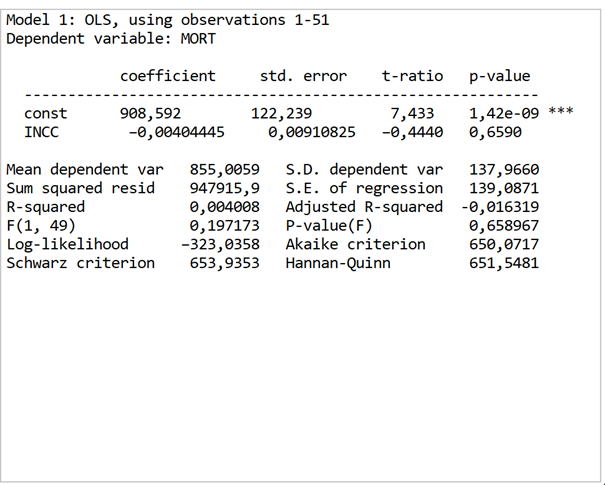
\includegraphics{images/Bilde3.png}

\includegraphics[width=1.67708in,height=0.16667in]{assignment_gretl_files/mediabag/wNtCyln93qMNgAAAABJR.png}

\includegraphics[width=1.85417in,height=\textheight]{assignment_gretl_files/mediabag/8PJUTcKBj9OuMAAAAASU.png}

The model is estimated to use 51 observations. The estimated intercept
is 908,592 and the coefficient for income (INCC) is --0,00404. The
R-squared is 0,0040 and the F-statistic is 0,197 with a p-value of
0,659. \newpage{}

\textbf{2B:}

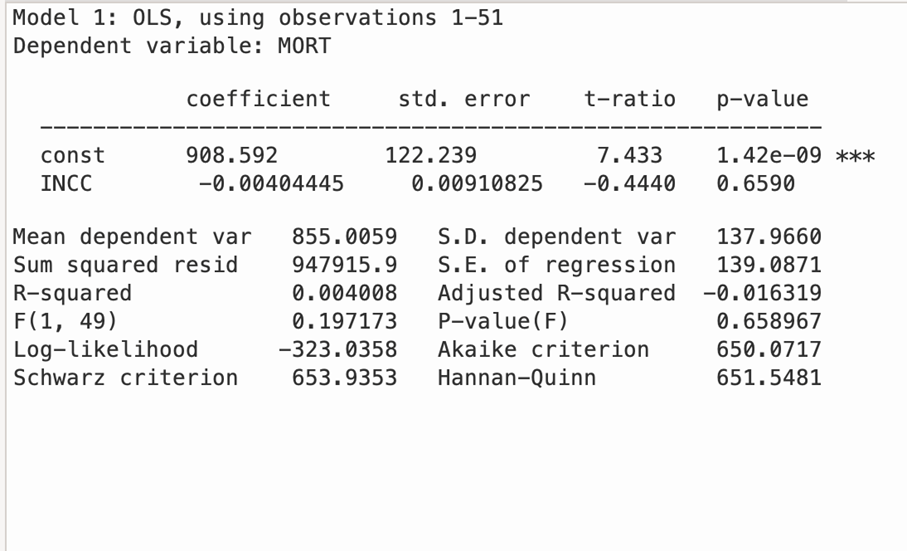
\includegraphics{images/Bilde4.png}

When INCC is 0, expected mortality is 908.592 (ß0). Since an income
level of zero is outside the realistic range of the data, the intercept
mainly serves as a technical component that determines where the
regression line crosses the vertical axis. The interesting parts comes
in the coefficient of INCC (ß1). The coefficient of INCC measures the
change in mortality associated with a one-unit increase in income. A one
unit increase in income reduces the predicted mortality rate by 0.004
units, holding everything else constant.

Mathematically:

Expect that income increases by 1000 units:
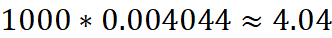
\includegraphics[width=1.44792in,height=\textheight]{images/clipboard-3821177194.png}

The model suggests a negative relationship between income and mortality.
A higher income is associated with lower mortality. Which is the public
conception, which is based on that higher income can afford better
quality food. In the US where health insurance is necessary for good
healthcare. \newpage{}

\textbf{2c)}

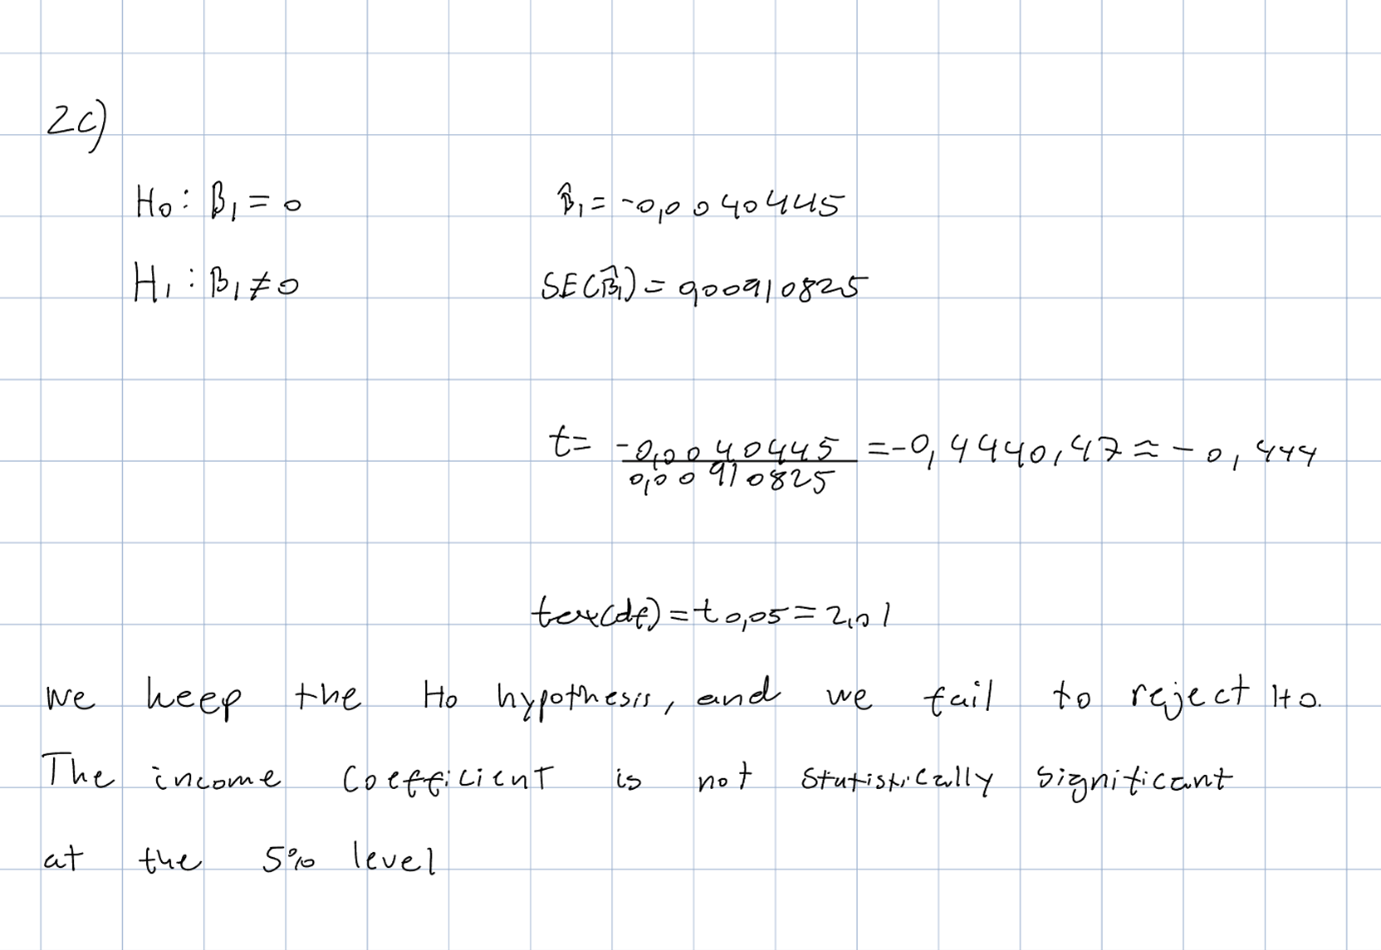
\includegraphics{images/Bilde5.png} \newpage{}

\textbf{2d)} From the summary statistics table:
~\includegraphics[width=2.41667in,height=\textheight]{assignment_gretl_files/mediabag/wPjWv8VgjX2SQAAAABJR.png}

INCC represents income per capita, measured in U.S. dollars for each
state.

In our dataset:

INCC min = 9187

INCC mean = 13249

INCC max = 18187

Substitute into the equation:

When INCC = 9187:
\includegraphics[width=3.19792in,height=\textheight]{assignment_gretl_files/mediabag/8HMdAhEeWBlc0AAAAASU.png}

When INCC = 13249:
\includegraphics[width=1.02083in,height=0.1875in]{assignment_gretl_files/mediabag/x9egTbLEXubfAf2WBfwB.png}

When INCC = 18187:
\includegraphics[width=1.02083in,height=0.1875in]{assignment_gretl_files/mediabag/8AJraxO-uHcR4AAAAASU.png}

Using the estimated OLS model, we compute predicted mortality rates for
different levels of income (INCC). Predictions are reported for low
(min), average (mean), and high (max) income values observed in the
sample. \newpage{}

\textbf{2e)}


\includegraphics{images/Bilde6.jpg}

The prediction interval is quite large {[}569.035, 1139.147{]} which we
can also see in
\includegraphics[width=0.16667in,height=\textheight]{assignment_gretl_files/mediabag/IQ78F0Wz1gAAAABJRU5E.png}.
This means that the model explains pretty much none of the variation of
the mortality. That means that we can't use income as a regressor for
simple regression to explain what leads to a higher mortality rate.
\newpage{}

\section{3. Multiple regression}\label{multiple-regression}

\textbf{a)} Our dependent variable is still mortality. Our additional
variables are: INCC, AGED, TOBC and EDU2. INCC, per capita income, is
included as the main explanatory variable of interest.The reason for
choosing EDU2 over EDU1 as to complete 4 years of college, you would
have to complete high school or other equivalents. We expect that there
would be a minor difference between a college and no college education.
Economic theories and empirical research questions suggest that higher
incomes are associated with better access to healthcare and improved
living situations and healthier lifestyles. AGED, is the proportion of
the population aged over 65 years, is included because mortality rates
are naturally higher in states with older populations. Controlling for
age structures ensures that the estimated effect of income is simply
capturing demographic differences across states. TOBC, cigarette
consumption per capita, is included because smoking is a major risk
factor for mortality. Differences in smoking behavior across states may
influence mortality independently of income. EDU2, the proportion of the
population completing 4 or more years of college, is included as a proxy
for human capital and health related behavior.~ Higher education levels
are generally associated with better health awareness, better access to
healthcare and healthier lifestyles. Including these variables allows
our coefficient on INCC to be interpreted as the partial effect of
income on mortality, holding age structure, smoking behavior, and
education constant. \newpage{}

\begin{enumerate}
\def\labelenumi{\alph{enumi})}
\setcounter{enumi}{1}
\tightlist
\item
\end{enumerate}

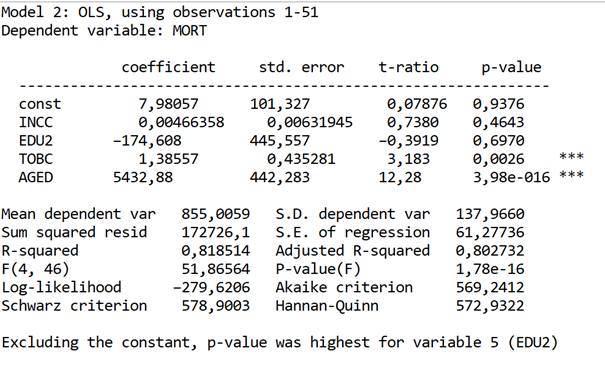
\includegraphics{images/Bilde7.png}

The multiple regression model is estimated by using 51 cross-sectional
observations with MORT as the dependent variable. The estimated
coefficients are:

INCC: 0.00466

EDU2: --174.61

TOBC: 1.3856

AGED: 5432.88

The model has an R-squared of 0.819 and an Adjusted R-squared of 0.803,
indicating that approximately 80\% of the variation in mortality across
states is explained by the included variables. This is a major
improvement over the previous situation with an R-squared of about
0,004.

The overall F-statistics are 51.87, with a p-value of 1.78e-16,
indicating that the model is jointly statistically significant at the
5\% level. \newpage{}

\textbf{c)} The coefficient on INCC is 0.00466. This implies that per
one dollar that ~increases in per capita, income is associated with an
increase of 0.00466 in the mortality rate, holding other variables
constant. Interpreting this per \$1000 increase:~
\includegraphics[width=1.23958in,height=\textheight]{assignment_gretl_files/mediabag/zD1cUmZ4AAAAASUVORK5.png}\emph{\hfill\break
}

Thus, a \$1000 increase in per capita income is associated with an
increase of approximately 4.66 deaths per 100,000 population, holding
age structure, smoking, and education constant. However, this effect
must be evaluated in terms of statistical significance.

The coefficient on EDU2 is --174.61. Since EDU2 is measured as a
proportion, a 0.01 (one percentage point) increase in the share of
college-educated individuals changes mortality by:
\includegraphics[width=1.5in,height=\textheight]{assignment_gretl_files/mediabag/wBn3dS90apHUQAAAABJR.png}

Thus, a one percentage point increase in college education is associated
with a reduction of approximately 1.75 deaths per 100,000 population,
holding other factors constant.

The coefficient on TOBC is 1.3856, indicating that higher cigarette
consumption is associated with higher mortality. A one-unit increase in
cigarette consumption increases predicted mortality by approximately
1.39 deaths per 100,000 population, holding other variables constant.

The coefficient on AGED is 5432.88. Since AGED is measured as a
proportion, a 0.01 (one percentage point) increase in the share of the
population over 65 increases mortality by:
\includegraphics[width=1.53125in,height=\textheight]{assignment_gretl_files/mediabag/fHUlndH68MHVNbcia6HR.png}

Thus, a one percentage point increase in the elderly population is
associated with approximately 54 additional deaths per 100,000
population, holding other variables constant. This is as expected as
most common source of death in the US in 2023 was heart disease
(National Center for Health Statistics, u.d.), and its more prevalent in
the older population (Maddalena Lettino, 2022). If we also consider our
everyday life and situation we most often hear of elderly people passing
away. It thus provides further evidence for our everyday belief of older
age being the largest contributor to old age.

\newpage{}

\textbf{d)}

To evaluate the statistical significance of the independent variables,
we examine their p-values at the 5\% significance level. A variable is
considered statistically significant if its p-value is below 0,005.

From the regression results, the variables TOBC and AGED are
statistically significant, with p-values of 0,0026 and 3,98e-16
respectively. This indicates that cigarette consumption and the
proportion of the population over age 65 have a statistically
significant association with mortality rates across states.

In contrast, the variables INCC and EDU2 have p-values of 0,04643 and
0,6970, which are both greater than 0,05. Therefore, we fail to reject
the null hypothesis that their coefficients are equal to zero. This
suggests that income per capita and the share of college-educated
individuals do not have statistically significant effect on mortality in
this model.

\textbf{e)} Compared to the simple regression model, the multiple
regression model provides a substantially better fit. In the simple
regression, where mortality was explained only by income, the R-squared
was approximately 0,004, indicating that income alone explained almost
none of the variation in mortality across states.

In the multiple regression model, the R-squared increases to 0,819,
meaning that approximately 81,9\% of the variation in mortality rates
can be explained by the included variables. This suggests that mortality
is influenced by several socioeconomic and health-related factors than
income alone.

We also saw the effect of omitted variable bias when going from a simple
regression to a multiple regression. We saw that there was a change from
a negative value to a positive one. The bias that where prevalent in
this set is negative due to the slope-coefficient in simple regression
being negative subtracted by the positive multiple regression slope,
giving a final negative value, and thus and negative bias. Another
factor to consider is that in states with an older population there is
likely an higher income as well.

The inclusion of variables such as cigarette consumption and the share
of elderly population significantly improves the explanatory power of
the model, highlighting the importance of considering multiple
determinants when analyzing moratity differences across states.
\newpage{}

\section{4.1 Dummy Variable Analysis}\label{dummy-variable-analysis}

\textbf{A)} We saw that income had a negative effect on mortality. Now
we want to find out if there is a threshold where it changes? Therefore,
we made a dummy variable where we set the mean as the threshold for
effect the dummy variable. The mean where 13249.2, and it was set to be
higher than mean income. We have seen that if the income is higher.

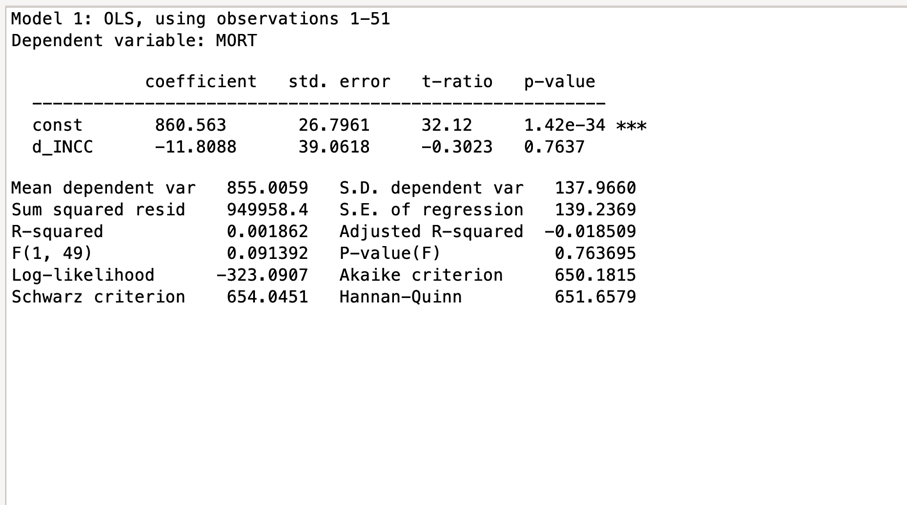
\includegraphics{images/Bilde8.png}

We can see that a higher income than the mean will lead to a lower
mortality. But this is insignificant as seen p the p-value being higher
than the significance level of 0,05. With our significance level of 76\%
there is a large chance that the relationship between the dummy variable
and income occurred by chance. We can therefore not conclude that the
income threshold as an effect on the dependent variable. We therefore
must add control variables to conclude if that it is income alone that
drives the lower mortality, or if its other factors that tend to occur
in high income states. The control variables we want to have a look at
is proportion of population over 65 (AGED), poverty (POV) and per-capita
health expenditure by state (HEXC).

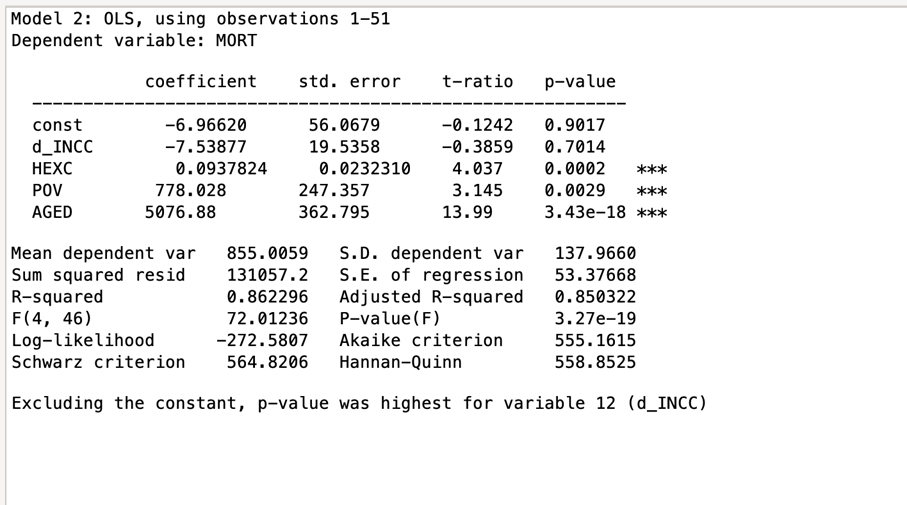
\includegraphics{images/Bilde9.png}

We can directly see that it these variables that have the biggest impact
on mortality. With the control variables we can now account for 86\% of
the variation of the model. The model flags our dummy variable, since
it's having the biggest p-value for a non-constant.~ We can therefore
see that an income threshold doesn't have an significant effect on
mortality. The other control variables do though, where age has the
biggest effect. We wanted to have a further look at it and found that
76\% of the variation is explained by age alone.

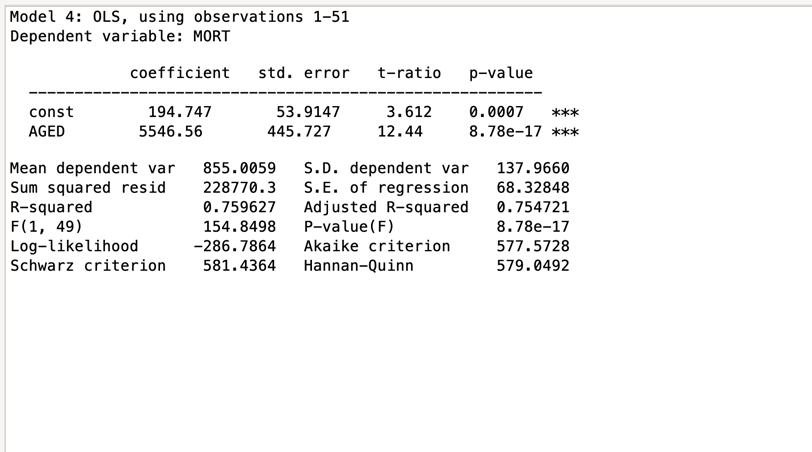
\includegraphics[width=4.70833in,height=\textheight]{images/Bilde10.png}

This is quite ordinary, due to most death reporting's in this health
groups being from age-related diseases. \newpage{}

\textbf{b)} The dummy variable was constructed to test whether states
with income above the sample mean have systematically different
mortality rates compared to states with income below the mean. The
threshold was set at the mean income level of 13~249,2. The dummy
variable therefore takes the value 1 for states with income above the
mean and 0 otherwise. The regression results indicate that the
coefficient for the income dummy variable is not statistically
significant. The p-value associated with the dummy variable is higher
than the 5\% significance level, meaning that we fail to reject the null
hypothesis that the dummy coefficient is equal to zero. This implies
that there is no statistical evidence that states with income above the
mean, when the dummy variable is considered on its own. When additional
control variable is included in the model, such as the share of the
population over 65 years (AGED), poverty rates (POV), and per-capita
healthcare expenditure (HEXC), the explanatory power of the model
increases substantially. The R-squared rises to approximately 0.86,
indicating that these variables collectively explain a large portion of
the variation in mortality across states. However, even after
controlling for these factors, the income dummy variable remains
statistically insignificant.

This suggests that the observed differences in mortality rates between
stats are not primarily driven by whether income is above or below the
mean threshold. Instead, demographic factors, particularly the
proportion of elderly individuals in the population, appear to play a
much more important role. Age structure has the strongest impact on
mortality rates, which is consistent with the fact that mortality
naturally increases with age. To test this, we made a new dummy variable
were wanted to how much of the model is explained by an age. We
therefore made a dummy variable where the threshold is an age above the
median. With this dummy variable we found that 40\% of the model is
explained by the dummy variable.

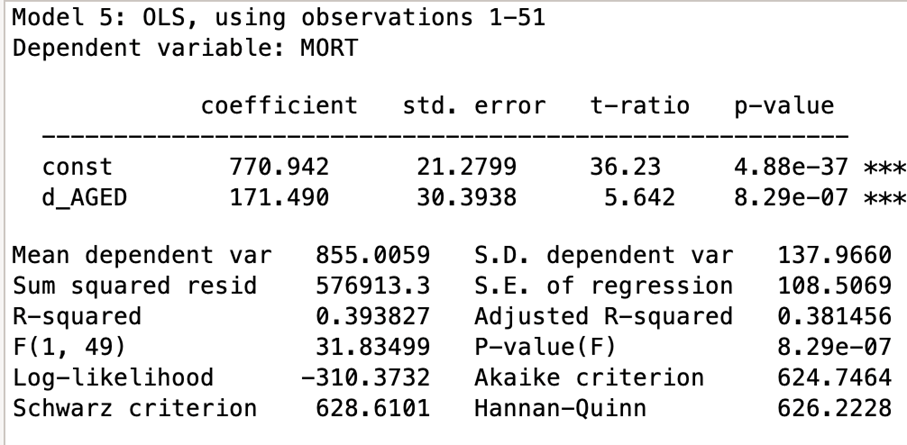
\includegraphics[width=2.95833in,height=\textheight]{images/Bilde11.png}

We can therefore see that aged is one of the major factors for
explaining mortality. ~We can also see that the states in with an age
above the median has an higher mortality rate by 171.49, which provides
further evidence for age being the major factor for explaining
mortality. The P-value is also significant which provides evidence for
that age being a factor in mortality.

An interaction effect would be relevant if the relationship between
income and mortality differed systematically between high- and
low-income states. However, since the dummy variable itself was not
statistically significant, adding an interaction term would further
complicate the RQ without adding a meaningful explanation. ~A fixed
effect specification was therefore considered sufficient for the purpose
of this analysis.

In conclusion, the dummy variable analysis does not provide evidence
that an income threshold effect exists in this dataset. Mortality
differences across states are better explained by demographic and
health-related variables rather than by a simple high-income versus
low-income classification. We found evidence for this through the dummy
variable created for age above the median. \newpage{}

\section{5. Model selection and
Analysis}\label{model-selection-and-analysis}

\textbf{a)} The different regression models can be used to predict
mortality rates for given values of the explanatory variables. In the
simple regression model, mortality is explained only by income (INCC).
However, the results from this model show that income alone does not
explain much of the variation in mortality across states. The R-squared
is around 0.004, which means that the model explains almost none of the
variation in the dependent variable. Because of this, predictions from
the simple regression model are quite unreliable and the model does not
give a very good explanation of mortality differences between states.

In the multiple regression model, several additional variables were
included in order to better explain mortality rates. The model includes
income (INCC), the proportion of the population over 65 years (AGED),
cigarette consumption (TOBC), and the proportion of the population with
four or more years of college education (EDU2). By including these
variables, the model considers both demographic factors and
health-related behavior. This model has a much higher explanatory power,
with an R-squared of 0.819, meaning that about 81.9\% of the variation
in mortality rates across states can be explained by the variables in
the model. This also means that predictions from this model are more
reliable compared to the simple regression.

In the dummy variable model, states were divided into two groups
depending on whether their income was above or below the sample mean.
The idea was to test if there was some kind of threshold effect for
income. However, the results show that the dummy variable is not
statistically significant. This suggests that simply separating states
into high-income and low-income groups does not explain mortality
differences in a meaningful way. \newpage{}

\textbf{b)} Based on the results from the analysis, the multiple
regression model seems to be the most appropriate model for predicting
mortality rates.

The simple regression model performs poorly because it only includes
income as an explanatory variable. Mortality is influenced by many
different factors, and income alone is clearly not enough to explain the
variation across states. We therefore have met the effect of omitted
variable bias --- this occurs when excluded variables, such as age
distribution, smoking habits and education level, both affect mortality
and are correlated with income. As a result, the coefficient on income
absorbs the effect of these missing variables, which is also reflected
in the very low R-squared value.

The dummy variable model also does not perform as well as the multiple
regression model. Even though it tries to capture differences between
higher-income and lower-income states, the results show that the dummy
variable is not statistically significant. This indicates that the
threshold effect of income does not seem to play an important role in
explaining mortality differences.

The multiple regression model, on the other hand, includes several
variables that are likely to influence mortality. In particular, the
proportion of elderly people and cigarette consumption appear to have
strong effects on mortality rates. The model also has a much higher
R-squared value compared to the other models. Because of this, the
multiple regression model provides a better and more realistic
explanation of mortality differences across states.

Overall, the multiple regression model seems to give the most reliable
predictions and therefore it is the preferred model in this analysis.

\section{Bibliography}\label{bibliography}

Maddalena Lettino, J. M. (2022, Februar 15). \emph{Cardiovascular
disease in the elderly: proceedings of the European Society of
Cardiology---Cardiovascular Round Table - Oxford Academic}. Hentet fra
Oxford Academic:
https://academic.oup.com/eurjpc/article/29/10/1412/6529006

National Center for Health Statistics. (u.d.). \emph{FastStats - Leading
Causes of Death}. Hentet Mars 15, 2026 fra FastStats:
https://www.cdc.gov/nchs/fastats/leading-causes-of-death.htm

Kivedal, B.K (2023) \emph{Anvendt Statistikk og Økonometri} (1. utgave).
Universitetsforlaget.




\end{document}
